\section{Durchführung}

Der experimentelle Aufbau ist in Abbildung \ref{abb:aufbau} zu sehen. Ein kollimierter $^{137}$Cs-Strahl wird auf einen $\SI{3}{\centi\meter}\times\SI{3}{\centi\meter}\times\SI{3}{\centi\meter}$ Würfel, der aus $\num{3}\times\num{3}\times\num{3}$ einzelnen Elementarwürfel besteht, geschossen und von einem NaJ-Detektor detektiert. Die erzeugten Pulse werden verstärkt und von einem Multichannelanalyzer in verschiedene Energie-Bins eingeteilt.

\begin{figure}
    \centering
    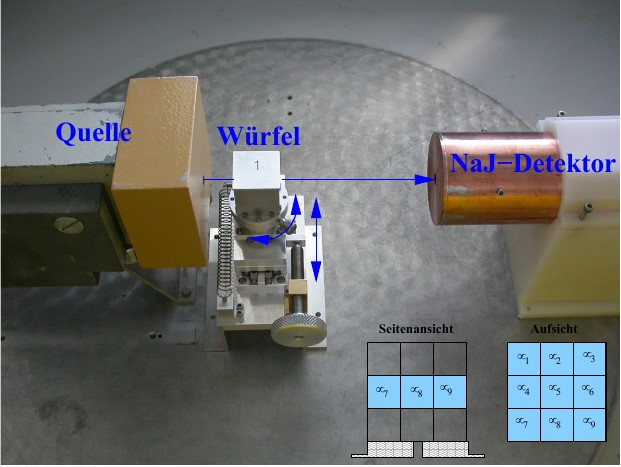
\includegraphics[width=0.7\textwidth]{figures/aufbau.jpg}
    \caption{Der Aufbau des Tomografie Versuchs ist hier gezeigt. Links ist die $^{137}$Cs Quelle, in der Mitte der Würfel und rechts der NaJ-Detektor. \cite{anleitung}}
    \label{abb:aufbau}
    \end{figure}

Insgesamt gibt es fünf verschiedene Würfel, die alle mit einer Aluminiumhülle von \SI{1}{\milli\meter} umschlossen sind. Die Würfel 2 und 3 beinhalten jeweils verschiedene Materialien, während Würfel 5 zwei verschiedene Materialien enthält. 

Das Programm \textit{winTMCA32} ist dabei das grafische Interface, das genutzt wird, um den Detektor zu kontrollieren und dessen Messungen aufzunehmen und zu speichern. 
Die Detektorspannung liegt bei $U_\text{Detektor} = \SI{1}{\kilo\volt}$, der Verstärkungsfaktor bei $V_\text{Fein}=\num{1.5}$. 

Als erstes wird eine Messung des Spektrums ohne Probe durchgeführt und der Bereich des Photopeaks wird bestimmt.  
Anschließend werden die Würfel 1 bis 3 eingesetzt und am Ende der Würfel 5. 

Für die Würfel 1 bis 3 wird in den drei gleichen Richtungen mit jeweils \SI{200}{\second} pro Richtung gemessen. 
Für den Würfel 5 wird in zwölf verschiedene Richtungen mit jeweils \SI{300}{\second} pro Richtung gemessen.
Die jeweiligen Richtungen mit denen gemessen wurde sind in \ref{abb:richtungen} beschrieben. Würfel 1 bis 3 sind dabei in Richtung $I_2, I_3, I_5$ gemessen worden und Würfel 5 in alle zwölf Richtungen. 

\begin{figure}
    \centering
    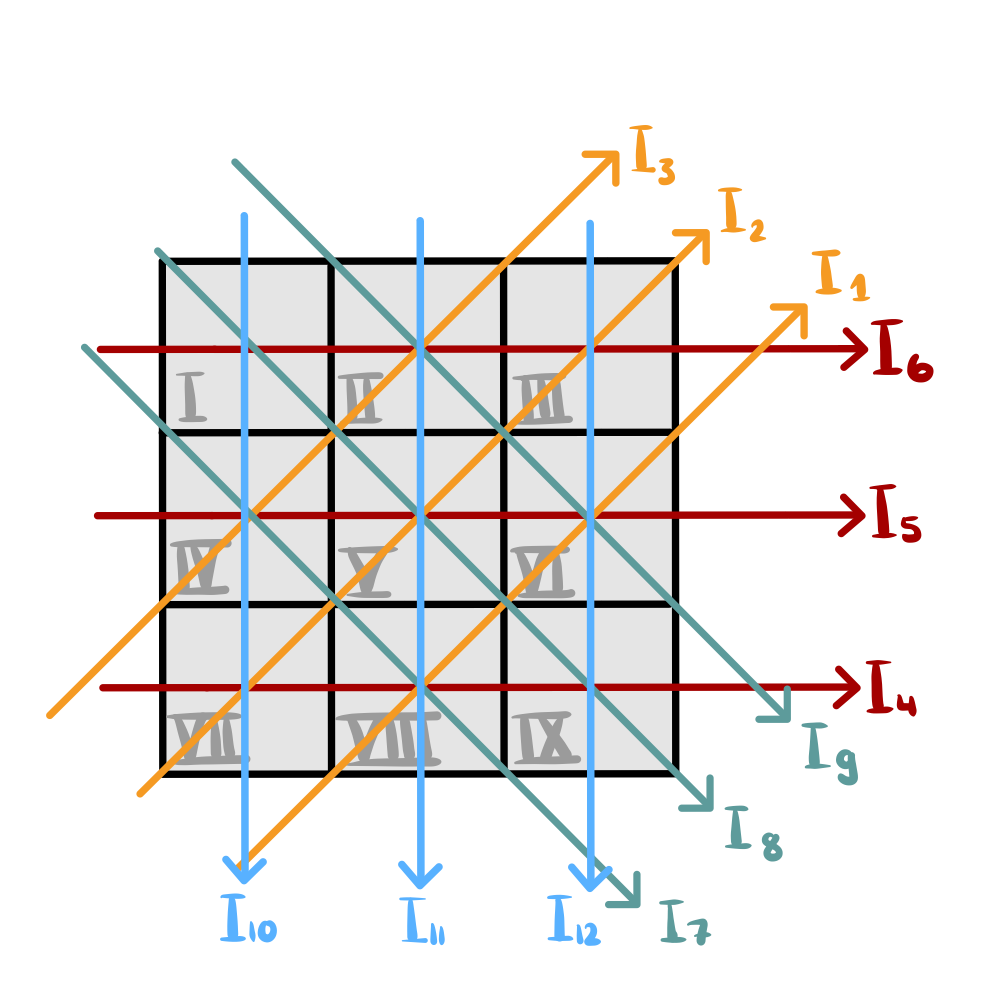
\includegraphics[width=0.7\textwidth]{figures/richtungen.jpeg}
    \caption{Die Einzelnen Projektionsrichtungen sind hier für die Würfel in 2D gezeigt. Analog zu dieser Beschriftungen wird gemessen.} 
    \label{abb:richtungen}
\end{figure}